\chapter{RL for {\sc ltl}$_f$/{\sc ldl}$_f$ Rewards}
\label{ch:rl}

In this chapter, we discuss Reinforcement Learning with non-Markovian rewards specified by \LLf formulas. The main contribution of this chapter is to devise a natural extension of the construction proposed in \citep{AAAI1817342} for a reinforcement learning task. That is, we show that it is possible to do reinforcement learning for non-Markovian rewards, expressed in \LLf formulas, by expanding the state space of the agent from the automata associated to the \LLf reward formulas.


\section{Reinforcement Learning}
\label{RL}
Reinforcement Learning \citep{Sutton:1998:IRL:551283} is a sort of optimization problem where an \emph{agent} interacts with an \emph{environment} and obtains a \emph{reward} for each action he chooses and the new observed state. The task is to maximize a numerical reward signal obtained after each action during the interaction with the environment. The agent does not know a priori how the environment works (i.e. the effects of his actions), but he can make observations in order to know the new state and the reward. Hence, learning is made in a \emph{trial-and-error} fashion. Moreover, it is worth to notice that in many situation reward might not be affected only from the last action but from an indefinite number of the previous actions. In other words, the reward can be \emph{delayed}, i.e. the agent should be able to foresee the effect of his actions in terms of future expected reward. Figure \ref{fig:agent-environment} represent the interaction between the agent and the environment in this setting.
\begin{figure}[!h]
	\centering
	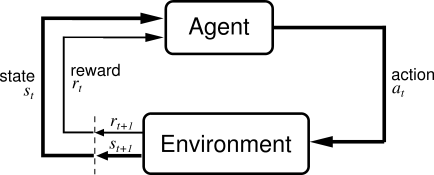
\includegraphics[width=.8\linewidth]{images/agent-environment}
	\caption{The agent and its interaction with the environment in Reinforcement Learning}\label{fig:agent-environment}
\end{figure}

In the next subsections, we introduce some of the classical mathematical frameworks for RL: Markov Decision Process (MDP) and Non-Markovian Reward Decision Process (NMRDP).
\section{Markov Decision Process (MDP)}
\label{MDP}

A Markov Decision Process (MDP) $\MDP$ is a tuple $\tup{\States, \Actions, \TrFun, \Reward, \DiscFact}$ containing a set of \emph{states} $\States$, a set of \emph{actions} $\Actions$, a \emph{transition function} $\TrFun: \States \times \Actions \to Prob(\States)$ that returns for every pair state-action a probability distribution over the states, a \emph{reward function} $\Reward: \States \times \Actions \times \States \to \Reals$ that returns the reward received by the agent when he performs action $a$ in $s$ and transitions in $s'$, and a \emph{discount factor} $\DiscFact$, with $0 \le \DiscFact \le 1$, that indicates the present value of future rewards. With $\TrFun(s, a, s')$ we denote the probability to end in state $s'$ given the action $a$ from $s$.

The discount factor $\DiscFact$ deserves some attention. Its value highly influences the MDP, its solution, and how the agent interprets rewards. Indeed, if $\DiscFact = 0$, we are in the pure \emph{greedy} setting, i.e. the agent is shortsighted and looks only at the reward that it might obtain in the next step, by doing a single action. The higher $\DiscFact$, the longer the sight horizon, or the foresight, of the agent: the far rewards are taken into account for the current action choice. If $\DiscFact < 1$ we are in the \emph{finite horizon} setting: namely, the agent is intrinsically motivated to obtain rewards as fast as possible, depending on how $\DiscFact$ is far from $1$. When $\DiscFact = 1$ we are in the \emph{infinite horizon} setting, which means that the agent considers far rewards as they can be obtained in the next step. In other words, we may think the agent as \emph{immortal}, since the time the agent spend to reach rewards does not matter anymore.

\medskip
A \emph{policy} $\Policy: \States \to \Actions$ for an MDP $\MDP$ is a mapping from states to actions, and represents a solution for $\MDP$. Given a sequence of rewards $\Reward_{t+1}, \Reward_{t+2}, \dots, \Reward_{T}$, the \emph{expected discounted return} $\ExpRet_t$ at time step $t$
is defined as: 
\begin{equation}\label{def:expected-discounted-return}
\ExpRet_t \defeq \sum_{k=t+1}^T \DiscFact^{k-t-1}\Reward_k
\end{equation} where can be $T = \infty$ and $\DiscFact = 1$ (but not both). 

The \emph{value function} of a state $s$, the \emph{state-value function} $\ValFun_\Policy(s)$ is defined as the expected return when starting in $s$ and following policy $\Policy$, i.e.:
\begin{equation}
\label{def:state-value-fun}
\ValFun_\Policy(s) \defeq \mathbb{E}_{\Policy}[\ExpRet_t | \States_t = s], \forall s \in \States
\end{equation}

Similarly, we define $\qFun_\Policy$, the \emph{action-value function for policy $\Policy$}, as:
\begin{equation}
\label{def:action-value-fun}
\qFun_\Policy(s, a) \defeq \mathbb{E}_{\Policy}[\ExpRet_t | \States_t = s, \Actions_t = a], , \forall s \in \States, \forall a \in \Actions
\end{equation}

Notice that we can rewrite \ref{def:state-value-fun} and \ref{def:action-value-fun} recursively, yielding the \emph{Bellman equation}:

\begin{equation}
\label{def:bellman-state-value-fun}
\ValFun_\Policy(s) =  \sum_{s'} P(s' | s,a)[\Reward(s,a,s') + \DiscFact \ValFun(s')] 
\end{equation}

where we used the definition of the transition function:
\begin{equation}
\TrFun(s,a,s') = P(s' | s,a)
\end{equation}

We define the \emph{optimal state-value function} and the \emph{optimal action-value function} as follows:
\begin{equation}
\label{optimal-state-value-fun}
\ValOptFun(s)  \defeq \max_\Policy  \ValFun_\Policy(s), \forall s\in \States		
\end{equation}

\begin{equation}
\label{optimal-action-value-fun}
\qOptFun(s, a) \defeq \max_\Policy  \qFun_\Policy(s, a), \forall s\in \States, \forall a\in \Actions
\end{equation}

Notice that with \ref{optimal-state-value-fun} and \ref{optimal-action-value-fun} we can show the correlation between $\ValOptFun_\Policy(s)$ and $\qOptFun_\Policy(s, a)$:

\begin{equation}
\qOptFun(s, a) = \mathbb{E}_\Policy[R_{t+1} + \DiscFact \ValOptFun_\Policy(\States_{t+1})| \States_t = s, \Actions_t = a]
\end{equation}


We can define a partial order over policies using value functions, i.e. $\forall s\in \States. \Policy \ge \Policy' \iff \ValFun_\Policy(s) \ge \ValFun_{\Policy'}(s)$. 
Now we give the definition of optimal policy:
\begin{definition}\label{def:optimal-policy}
	An \emph{optimal policy} $\OptPolicy$ is a policy such that $\OptPolicy \ge \Policy$ for all $\Policy$. 
\end{definition}

Given an MDP $\MDP$, a typical reinforcement learning problem is the following: find an optimal policy for $\MDP$, without knowing $\TrFun$ and $\Reward$. Notice that instead of explicit specification of the transition probabilities and rewards, the transition probabilities are accessed through a simulator that is restarted many times from a fixed or uniformly random initial state $s_0\in\States$. We call this way of structuring the learning process \emph{episodic reinforcement learning}. Usually, in episodic reinforcement learning, we require the presence of one or more \emph{goal states} where the simulation of the MDP ends and the task is considered completed, or a maximum time limit $T$ for the number of actions that can be taken by the agent in one single episode, and the overcoming of $T$ determines the end of the episode. Optionally, \emph{failure states} can be also defined, where the episode ends similarly to goal states, but the task is considered failed.

\subsubsection{Examples}
Many dynamic systems can be modeled as Markov Decision Processes. 

\begin{example}[\textbf{Gridworld}]\label{exa:gridworld} Perhaps the most simple MDP used as a toy example is \emph{Gridworld}, depicted in Figure \ref{fig:gridworld}.
There are $3\times 4$ cells, i.e. states of the MDP $\States = \set{s_{11}, s_{12}, \dots, s_{34}}\setminus \set{s_{22}}$. The agent can do four actions: $A = \set{Right, Left, Up, Down}$. The initial state is fixed and is $s_0 = s_{11}$ and the agent can move in any of the adjacent and free cells from the current state. Assuming an episodic task, the goal is to reach $s_{34}$, and $s_{24}$ represent a failure state. The state transition function $\TrFun$ can be \emph{deterministic}, i.e. the agent always succeeds in performing actions, or non-deterministic, i.e. the effect of an action is determined by the probabilistic distribution returned by $\TrFun(s, a)$. An example of non-deterministic $\TrFun$ is to give $90\%$ of success (the agent moves in the chosen direction) and $10\%$ of fail (the agent moves at either the right or left angle to the intended direction). If the move would make the agent walk into a wall (borders of the grid and $s_{22}$), the agent stays in the same place as before. The reward function $R(s,a,s')$ is defined as $-1$ if $s'=s_{24}$, as $1$ if $s'=s_{34}$, and $-0.01$ otherwise. The small negative reward given at each transition is a popular mean for reward function design: it is called \emph{step reward} and its purpose is to encourage the agent to finish the episode as fast as possible, with a priority proportional to the absolute value of the reward. The discount factor $\DiscFact$ should be strictly higher than 0 because more than one step is needed to reach the goal state.
	
\begin{figure}[h]
	\centering
	\caption{The Gridworld environment}\label{fig:gridworld}
	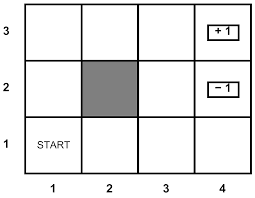
\includegraphics[width=.4\linewidth]{images/gridworld}
\end{figure}

An example of an optimal policy is shown in Figure \ref{gridworld-optimal-policy}. As the reader can notice, the arrows represent the action that should be taken in a certain cell, in order to maximize the expected return. We observe that the optimal action in $s_{13}$, according to the policy, is not the one to take the shortest path to the goal, i.e. the $Up$ action	. This is because there is a small probability to ens in $s_{24}$, the failure state, and be punished with a high negative reward. In terms of expected reward, it is better to take the longer path, at the price of collect small negative rewards, but avoiding the risk to fail miserably.
\begin{figure}
	\centering
	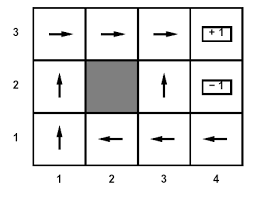
\includegraphics[width=.4\linewidth]{images/gridworld-optimal-policy}
	\caption{An example of optimal policy for the Gridworld environment}\label{gridworld-optimal-policy}. 
\end{figure}

\end{example}

\begin{example}[\textbf{Breakout}]\label{exa:breakout}
	Breakout is a well-known arcade video game developed by Atari. In this work, we implemented a clone of the original Breakout. Figure \ref{fig:breakout} shows a screenshot of the game. On the screen, there is a paddle at the bottom, many bricks at the top arranged in a grid layout with $n$ rows and $m$ columns (in the figure $3\times 3 = 9$ bricks), and a ball that is free to move across the screen. The ball bounces when it hits a wall, a brick or the paddle. When the ball hits a brick, that brick is broke down and is removed from the screen. The paddle (the agent) can move left, move right or do nothing. The \emph{goal} is to remove all the bricks while avoiding that the paddle misses the rebound of the ball (\emph{failure}).
	
	The relevant features are: position of the paddle $p_x$, position of the ball $b_x, b_y$, speed of the ball $v_x, v_y$ and status of each brick (booleans) $b_{ij}$. This features of the system gives all the needed information to predict the next state from the current state. Hence we can build an MDP where: $\States$ is the set of  all the possible values of the sequence of features $\tup{p_x, b_x, b_y, v_x, v_y, b_{11}, \dots, b_{nm}}$, $\Actions = \set{Right, Left, No\-op}$, transition function $\TrFun$ determined by the rules of the game. We give reward $R(s,a,s')=10$ if a particular brick in $s'$ has been removed for the first time, plus $100$ if that brick was the last (i.e. goal reached).
	\begin{figure}[h]
		\centering
		
\includegraphics[width=.6\linewidth]{images/breakout.jpg}
		\caption{A screenshot from the video game \Breakout}\label{fig:breakout}. 
	\end{figure}
	\paragraph{Violation of the Markov property considering a smaller set of features:}
	Notice that considering a strict subset of the set of features for $\States$ leads to violating the Markov property of $\TrFun$. Indeed, consider the case when we remove $v_x$ and $v_y$ from the set of features. In this setting, we removed the pieces of information about the dynamics of the system. More precisely, we cannot predict, knowing only the current state, the value of the features $b_x$ and $b_y$ for the next step, because we do not know where the ball is going (up-left, down-right and so on). In order to correctly predict the next position of the ball, we should know whether earlier in the episode the ball was coming from the bottom or from the top. But this fact clearly shows that the Markovian assumption is violated. Similar arguments apply in the case where we remove the status of the bricks $b_{11}, \dots, b_{nm}$: indeed, if the ball in the next step is near to a brick, knowing about the status of the brick is determinant to predict if the ball will continue its trajectory (the case when the brick is absent) or it will break down the brick and bounce, changing the direction of its motion (the case when the brick is present).
	
\end{example}

\section{Temporal Difference Learning}
\label{sect:temporal-difference-learning}
\emph{Temporal difference learning} (TD) \citep{Sutton1988} refers to a class of model-free reinforcement learning methods which learn by bootstrapping from the current estimate of the value function. These methods sample from the environment, like Monte Carlo (MC) methods, and perform updates based on current estimates, like dynamic programming methods (DP) \citep{Bellman:1957}. We do not discuss MC and DP methods here.

Q-Learning \citep{watkins1989learning, Watkins1992} and Sarsa are such a methods. They update $\qFunEst(s, a)$, i.e. the estimation of $\qOptFun(s, a)$ at each transition $(s, a) \to (s', r)$. The update rule is the following:
\begin{equation}\label{td-update-rule}
\qFunEst(s, a) \leftarrow \qFunEst(s, a) + \LRate \delta
\end{equation}
where $\delta$ is the \emph{temporal difference}. In Sarsa, it is defined as:
\begin{equation}\label{def:temporal-difference}
\delta = r + \DiscFact \qFunEst(s', a') - \qFunEst(s, a)
\end{equation}
whereas in Q-Learning:
\begin{equation}
\delta = r + \DiscFact \max_{a'} \qFunEst(s', a') - \qFunEst(s, a)
\end{equation}

TD$(\lambda)$ is an algorithm which uses \emph{eligibility traces}. The parameter $\lambda$ refers to the use of an eligibility trace. The algorithm generalizes MC methods and TD learning, obtained respectively by setting $\lambda = 1$ and $\lambda = 0$. Intermediate values of $\lambda$ yield methods that are often better of the extreme methods. 
Q-Learning and Sarsa that has been shown before can be rephrased with this new formalism as Q-Learning(0) and Sarsa(0), special cases of Watkin's Q$(\lambda)$ and Sarsa($\lambda$) respectively.
In this setting, Equation \ref{td-update-rule} is modified as follows:
\begin{equation}\label{td-lambda-update-rule}
\qFunEst(s, a) \leftarrow \qFunEst(s, a) + \LRate \delta e(s, a)
\end{equation}

Where $e(s, a) \in [0, 1]$, the \emph{eligibility of the pair $(s, a)$}, determines how much the temporal difference $\delta$ should be weighted.
Sarsa($\lambda$) is reported in Algorithm \ref{alg:sarsa-lambda}, whereas Watkin's Q($\lambda$) in Algorithm \ref{alg:q-learning-lambda}, both  in the variants using \emph{replacing eligibility traces} (see line \ref{sarsa-lambda-replacing-traces} and line \ref{q-learning-lambda-replacing-traces}, respectively).
\begin{algorithm}
	\caption{Sarsa($\lambda$) \citep{Singh:1996:RLR:225667.225679}}
	\label{alg:sarsa-lambda}
	\begin{algorithmic}[1]
		\State Initialize $Q(s, a)$ arbitrarily and $e(s, a)=0$ for all $s, a$
		
		\Repeat \{for each episode\} 
			\State initialize $s$
			\State Choose $a$ from $s$ using policy derived from $Q$ (e.g. $e$-greedy)
			\Repeat \{for each step of episode\}
				\State Take action $a$, observe reward $r$ and new state $s'$
				\State Choose $a'$ from $s'$ using policy derived from $Q$
				\State $\delta \gets r + \gamma Q(s', a') - Q(s, a)$
				\State $e(s, a) \gets 1$ \Comment{replacing traces} \label{sarsa-lambda-replacing-traces}
				\For{$\mathbf{all}\ s, a$}
					\State $Q(s, a) \gets Q(s, a) + \alpha\delta e(s, a)$
					\State $e(s, a) \gets \DiscFact\lambda e(s, a)$
				\EndFor
				\State $s\gets s'$, $a \gets a'$
			\Until state $s$ is terminal
		\Until
	\end{algorithmic}
	
\end{algorithm}
\begin{algorithm}
	\caption{Watkin's Q($\lambda$) \citep{watkins1989learning}}
	\label{alg:q-learning-lambda}
	\begin{algorithmic}[1]
		\State Initialize $Q(s, a)$ arbitrarily and $e(s, a)=0$ for all $s, a$
		\Repeat \{for each episode\} 
			\State initialize $s$
			\State Choose $a$ from $s$ using  policy derived from $Q$ (e.g. $e$-greedy)
			\Repeat \{for each step of episode\}	
				\State Take action $a$, observe reward $r$ and new state $s'$
				\State Choose $a'$ from $s'$ using policy derived from $Q$ (e.g. $e$-greedy)
				\State $a^* \gets \arg\max_a Q(s', a)$ (if $a'$ ties for max, then $a^* \gets a'$)
				
				\State $\delta \gets r + \gamma Q(s', a^*) - Q(s, a)$
				\State $e(s, a) \gets 1$ \Comment{replacing traces}\label{q-learning-lambda-replacing-traces}
				\For{$\mathbf{all}\ s, a$}
					\State $Q(s, a) \gets Q(s, a) + \alpha\delta e(s, a)$
					\If{$a' = a^*$}
						\State $e(s, a) \gets \DiscFact\lambda e(s, a)$
					\Else 
						\State $e(s, a) \gets 0$
					\EndIf
					
					\State $e(s, a) \gets \DiscFact\lambda e(s, a)$
				\EndFor
				\State $s\gets s'$, $a \gets a'$
			\Until state $s$ is terminal
		\Until
	\end{algorithmic}
	
\end{algorithm}

\section{Non-Markovian Reward Decision Process (NMRDP)}\label{sect:NMRDP}
For some goals, it might be the case that the Markovian assumption of the reward function $\Reward$ -- that reward depends only on the current state, and not on history -- does not hold. Indeed, for many problems, it is not effective that the reward is limited to depend only on a single transition $(s,a,s')$; instead, it might be extended to depend on \emph{trajectories} (i.e. $\traj$), e.g. when we want to reward the agent for some (temporally  extended) behaviors, opposed to simply reaching certain states. 

This idea of rewarding behaviours has been proposed by \citep{bacchus1996rewarding} where they defined a new mathematical model, namely Non-Markovian Reward Decision Process (NMRDP), and showed how to construct optimal policies in this case.

In the next subsections, we give the main definitions to reason in this new setting. Then we show the solution proposed in \citep{bacchus1996rewarding}.

\subsection{Preliminaries}
Now follows the definition of NMRDP, which is similar to the MDP definition given in Section \ref{MDP}.

\begin{definition}\label{def:nmrdp}
	A Non-Markovian Reward Decision Process (NMRDP) \citep{bacchus1996rewarding} $\NMRDP$ is a tuple $\tup{\States, \Actions, \TrFun, \NMReward, \DiscFact}$ where $\States, \Actions, \TrFun$ and $\DiscFact$ are defined as in the MDP, and $\NMReward : \States^* \to \Reals$ is the \emph{non-Markovian reward function}, where $\States^* = \set{\projtraj_{n\ge0, s_i\in\States}}$ is the set of all the possible traces, i.e. projection of trajectories $\traj$
	
\end{definition}

Given a trace $\trace = \projtraj$, the \emph{value of $\trace$} is:
\begin{equation}
v(\pi) = \sum_{i=1}^{|\trace|} \DiscFact^{i-1}\NMReward(\projtraj)
\end{equation}
where $|\trace|$ denotes the number of transitions (i.e. of actions).

The policy $\NMPolicy$ in this setting is defined over sequences of states, i.e. $\NMPolicy: \States^* \to \Actions$. The \emph{value of $\NMPolicy$} given an initial state $s_0$ is defined as:

\begin{equation}
\ValFun^{\NMPolicy}(s) = \mathbb{E}_{\pi \sim \NMRDP, \NMPolicy, s_0}[v(\pi)]
\end{equation}

i.e. the expected value in state $s$ considering the distribution of traces defined by the transition function of $\NMRDP$, the policy $\NMPolicy$ and the initial state $s_0$.

We are interested in two problems, that we will study in the next sections:
\begin{itemize}
	\item Find an optimal (non-Markovian) policy $\NMPolicy$ for an NMRDP $\NMRDP$ (Definition \ref{def:nmrdp});
	\item Define the non-Markovian reward function for the domain of interest.
\end{itemize}

\subsection{Find an optimal policy $\NMPolicy$ for NMRDPs}\label{nmrdp-find-optimal-policy}
The  key  difficulty  with  non-Markovian rewards  is  that
standard optimization techniques, most based on Bellman's \citep{Bellman:1957} 
dynamic  programming  principle,  cannot be used. Indeed, this requires one to resort to optimization over a policy space that maps histories
(rather than states)  into actions, a process that would incur a great 
computational expense. \citep{bacchus1996rewarding} give the definition of 
a decision  problem \emph{equivalent} to an NMRDP  in  which  the  rewards  are
Markovian. This construction is the key element to solve our problem,
i.e. find an optimal policy for an NMRDP.


\subsubsection{Equivalent MDP}
Now we give the definition of \emph{equivalent} MDP of an NMRDP, and state an important result. 

\begin{definition}[\cite{bacchus1996rewarding}]
	\label{nmrdp-mdp-equivalence}
	An NMRDP $\NMRDP = \tup{\States, \Actions, \TrFun, \NMReward, \DiscFact}$ is \emph{equivalent} to an extended
	MDP $\MDP = \tup{\States', \Actions, \TrFun', \Reward', \DiscFact}$ if there exist two functions 
	$\tau: \States' \to \States$ and $\sigma: \States\to \States'$ such that
	\begin{enumerate}
		\item $\forall s \in \States: \tau (\sigma(s)) = s$; \label{nmrdp-mdp-equivalence-cond1}
		\item $\forall s_1, s_2 \in \States$ and $s_1' \in \States'$: if $\TrFun(s_1 , a, s_2 ) > 0$ and $\tau (s'_1) =
		s_1$, there exists a unique $s'_2 \in \States'$ such that $\tau (s'_2 ) = s_2$ and
		$\TrFun'(s'_1 , a, s'_2 ) = \TrFun(s_1, a, s_2 )$;
		\label{nmrdp-mdp-equivalence-cond2}
		\item For any feasible trace $\projtraj$ of $\NMRDP$
		and $\projtrajprime$ of $\MDP$ associated to the trajectories $\traj$ and $\trajprime$, such that $\tau(s'_i) = s_i$
		and $\sigma(s_0) = s'_0$, we have $R(\projtraj) =
		R'(s_{n-1}, a_{n-1}, s'_n)$.
		\label{nmrdp-mdp-equivalence-cond3}	
	\end{enumerate}
\end{definition}

Given the Definition \ref{nmrdp-mdp-equivalence}, we give the definition of corresponding policy:
\begin{definition}[\cite{bacchus1996rewarding}]\label{nmrdp-mdp-policy-equivalence}
	Let $\NMRDP$ be an NMRDP and let $\MDP$ be the equivalent MDP as defined in Definition \ref{nmrdp-mdp-equivalence}.
	Let $\Policy$ be  a  policy  for $\MDP$. The 
	\emph{corresponding policy} for $\NMRDP$ is  defined  as 
	$\NMPolicy(\tup{s_0, \dots, s_n}) = \Policy(s'_n) $,   where for the sequence $\tup{s'_0, \dots, s'_n}$ we have $\tau(s'_i) = s_i\ \forall i$ and $\sigma(s_0)=s'_0$
\end{definition}
From definitions \ref{nmrdp-mdp-equivalence} and 
\ref{nmrdp-mdp-policy-equivalence}, and since that for all 
policy $\Policy$ of $\MDP$ the corresponding policy 
$\NMPolicy$ of $\NMRDP$ is such that $ \forall s. \ValFun_\Policy(s) = \ValFun_{\NMPolicy}(\sigma(s))$, the following theorem holds:
\begin{theorem}[\cite{bacchus1996rewarding}]\label{nmrdp-mdp-equivalence-policy-optimality}
	Let $\Policy$ be an optimal policy for MDP $\MDP$. Then the corresponding policy is optimal for NMRDP $\NMRDP$.
\end{theorem}

The Theorem \ref{nmrdp-mdp-equivalence-policy-optimality} allows us to learn an optimal policy $\NMPolicy$ for NMRDP by learning a policy $\Policy$ over an equivalent MDP, which can be done by resorting on any off-the-shelf algorithm (e.g. see Section \ref{sect:temporal-difference-learning}). Moreover, obtaining the corresponding policy for the original NMRDP is straightforward, although in practice is not needed, since it is enough to run the policy $\Policy$ over the MDP.

In other words, the problem of finding an optimal policy for an NMRDP reduces to find an optimal policy for an equivalent MDP such that Condition 1, 2 and 3 of Definition \ref{nmrdp-mdp-equivalence} hold.


\subsection{Define the non-Markovian reward function $\NMReward$}
To  reward  agents  for  (temporally  extended)
behaviours, as opposed to simply reaching certain states, we need a way
to specify rewards for specific trajectories through the state
space. 
Specifying a non-Markovian reward function explicitly is quite hard and unintuitive, impossible if we are in an infinite-horizon setting. 
Instead, we can define \emph{properties} over trajectories and reward only the ones which satisfy some of them, in contrast to enumerate all the possible trajectories.

Temporal logics presented in Section \ref{sect:ltl} gives an effective way to do this. 
Indeed, in order to speak about a desired behavior,  i.e. fulfillment of properties that might change over time, we can define a \emph{formula} $\varphi$ (or more formulas) in some suited temporal logic formalism semantically defined over trajectories $\trace$, speaking about a set of properties $\Prop$ such that each state $s\in S$ is associated to a set of propositions ($S\subseteq 2^\Prop$). 
In this way, a trajectory $\trace = \traj$ is rewarded with $r_i$ iff $\trace \models \varphi_i$, where $r_i$ is the reward value associated to the fulfillment of behaviours signified by $\varphi_i$.

\subsection{Using \PLTL}
\label{sect:using-pltl}
In \citep{bacchus1996rewarding} the temporal logic formalism is \emph{Past Linear Temporal Logic} (\PLTL), which is a past version of \LTL (Section \ref{sect:ltl}).
As explained before, using the declarativeness of \PLTL, is possible to specify the desired behaviour (expressed in terms of the properties $\Prop$) that should be satisfied by the experienced trajectories and reward only them, hence obtaining a non-Markovian reward function. More formally, given a finite set $\Phi$ of \PLTL \emph{reward formulas}, and for each $\phi_i \in \Phi$ a real-valued reward $r_i$, the \emph{temporally extended reward function} $\bar{R}$ is defined as:
\begin{equation}\label{pltl-temp-extended-reward-fun}
\NMReward(\projtraj) = \sum_{\phi_i \in \Phi : \tup{s_0, s_1, \dots, s_n}\models \phi_i} r_i
\end{equation}


In order to run the actual learning task, \citep{bacchus1996rewarding} proposed a transformation from the NMRDP to an equivalent MDP with the state space \emph{expaneded} which allows to label each state $s\in \States$. The idea is that the labels should keep track in some way the (partial) satisfaction of the temporal formulas $\phi_i \in \Phi$. 
A state $s$ in the transformed state space is replicated multiple times, marking the difference between different (relevant) histories terminating in state $s$.

In this way, they obtained a compact representation of the required history-dependent policy
by considering only relevant history, and can produce this
policy using computationally-effective MDP algorithms.
In other words, the states of the NMRDP can be mapped into those of the expanded MDP, 
in such a way that corresponding states yield
same transition probabilities and corresponding traces have same rewards.


\section{RL for NMRDP with \LLf Rewards}\label{sect:nmrdp-llf-rewards}
In this section, we explain the main contribution of this chapter and one of the main contribution of the thesis. We devise a natural extension of the construction explained in \citep{AAAI1817342} for a reinforcement learning task. That is, we show that it is possible to do reinforcement learning for non-Markovian rewards, expressed in \LLf formulas, by applying an extension of the state space of the agent $\States$, analogously to the one described in Section \ref{sect:using-pltl}.
In the first section, we describe the approach proposed by \citep{AAAI1817342}; then, we observe that the expanded MDP can be used to do reinforcement learning to optimize \LLf non-Markovian rewards.

\subsection{NMRDP with \LTLf/\LDLf rewards}\label{sect:nmrdp-llf-rewards-small}
In this section, we explain how to specify non-Markovian rewards with \LTLf/\LDLf  formulas (instead of \PLTL) and how the associated MDP expansion works \citep{AAAI1817342}, analogously to what we saw with \PLTL (Section \ref{sect:using-pltl}).

The temporally extended reward function $\bar{R}$ is similar to Equation \ref{pltl-temp-extended-reward-fun}, but instead of using \PLTL formula we use \LLf formulas. Formally, given a set of pairs $\set{(\varphi_i, r_i)^m_{i=1}}$ (where $\varphi_i$ denotes the \LLf formula for specifying a desired behavior, and $r_i$ denotes the reward associated to the satisfaction of $\varphi_i$, and given a (partial) trace $\trace = \projtraj$, we define $\bar{R}$ as:
\begin{equation}
\NMReward(\trace) = \sum_{1\le i\le m: \trace \models \varphi_i} r_i
\end{equation}
For the sake of clarity, in the following we use $\set{(\varphi_i, r_i)^m_{i=1}}$ to denote $\bar{R}$.

Now we describe the MDP expansion for doing learning in this setting, as proposed in \citep{AAAI1817342}. 
Without loss of generality, we assume that every NMRDP $\NMRDP$ is reduced into another NMRDP $\NMRDP'=\tup{\States', \Actions', \TrFun', \Reward', \DiscFact}$:


\begin{gather}
	\begin{split}
	\States' &= \States\cup \set{s_{init}}\\
	\Actions' &= \Actions\cup \set{start}\\
	\TrFun'(s,a,s')  &=  \begin{cases}
			1 & \tm{if\ } s=s_{init}, a=start, s'=s_0\\
			0 & \tm{if\ } s=s_{init} \tm{and} (a\neq start \tm{or} s'\neq s_0)\\
			\TrFun(s, a, s') &  \tm{otherwise}\\
		\end{cases}\\
	\Reward'(\tup{s_{init}, s_0, \dots, s_n}) &= \Reward(\projtraj)
	\end{split}
	\label{def:nmrdp-with-dummy-initial-state}
\end{gather}

and $s_{init}$ is the new initial state. In other words, we prefix to every feasible trajectory $\NMRDP$ the pair $\tup{s_{init}, start}$, denoting the beginning of the episode. 
We do this for two reasons: allow to evaluate formulas in $s_0$ and make it compliant with the most general definition of the reward, namely $R(s, a, s')$, also when there is no true action that is done (i.e. empty trace).

\begin{definition}[\cite{AAAI1817342}]\label{nmrdp-mdp-transformation-brafman}
	Given an NMRDP $\NMRDP = \tup{S, A, \TrFun, \set{(\varphi_i, r_i)^m_{i=1}, \DiscFact}}$ (i.e. with non-Markovian rewards specified by \LLf formulas) it is possible to build an $\MDP = \tup{\States', \Actions, \TrFun', \Reward', \DiscFact}$ that is \emph{equivalent} (in the sense of Definition \ref{nmrdp-mdp-equivalence}) to $\NMRDP$. Denoting with 
	$\automaton_{\varphi_i} = \tup{2^\P, Q_i, q_{i0}, \delta_i,F_i}$ (notice that $S\subseteq 2^{\Prop}$ and $\delta_i$ is total) the \DFA associated 
	with $\varphi_i$ (see Section \ref{sect:llf2automata}), the equivalent MDP $\MDP$ is built as follows:
	\begin{itemize}
		\itemsep=0mm
		\item $S'=Q_1\times\cdots\times Q_m\times \States$ is the set of states;
		\item $\TrFun' : S'\times A \times S'\rightarrow [0,1]$ is defined as follows:
		\[
		\begin{array}{l}
		\Tr'(q_1,\ldots,q_m, s, a, q'_1,\ldots,q'_m, s') = {}\\
		\quad\left\{
		\begin{array}{ll}\label{tr-fun-expanded-mdp}
			Tr(s,a,s') &\mbox{if } \forall i:\delta_i(q_i,s') = q'_i\\
			0 & \mbox{otherwise}; 
			\end{array}\right.
		\end{array}
		\] 
		\item $R': S'\times A \times S'\rightarrow 
		\mathbb{R}$ is defined as:
		\[
		R'(q_1,\ldots,q_m, s, a, q'_1,\ldots,q'_m, s') = 
		%\sum_i \{\rew(\Phi_i) \mid \delta(q_i,t) \in F_i\} 
		\sum_{i: q_i'\in F_i} r_i
		\] 
	\end{itemize}
\end{definition}


\begin{theorem}[\cite{AAAI1817342}]\label{th:nmrdp-mdp-llf-equivalence}
	The NMRDP $\NMRDP= \tup{\States, \Actions, \TrFun, \{(\varphi_i,r_i)\}_{i=1}^{m}, \DiscFact}$ is equivalent to the  MDP $\MDP= \tup{\States',\Actions,\TrFun',\Reward', \DiscFact}$ defined in Definition \ref{nmrdp-mdp-transformation-brafman}.
\end{theorem}
\begin{proof}
	Recall that every $s' \in S'$ has the form $(q_1 ,\dots, q_m , s)$.
	Define $\tau(q_1 ,\dots, q_m, s) = s$. Define $\sigma(s) = (q_{10} ,\dots, q_{m0}, s)$.
	We have $\tau(\sigma(s)) = s$, hence Condition \ref{nmrdp-mdp-equivalence-cond1} is verified. Condition \ref{nmrdp-mdp-equivalence-cond2} of Definition \ref{nmrdp-mdp-equivalence} is easily verifiable by inspection. For Condition \ref{nmrdp-mdp-equivalence-cond3}, consider a possible trace
	$\trace = \projtraj$. We use $\sigma$ to obtain $s'_0 = \sigma(s_0)$
	and given $s_i$, we define $s'_i$ (for $1 \le i \le n$) to be the unique
	state $(q_{1,i} ,\dots, q_{m,i} , s_i)$ such that $q_{j,i} = \delta(q_{j,i-1}, s_i )$ for all
	$1 \le j \le m$. Moreover, we require that, without loss of generality, every trajectory in the new MDP starts from $s_{init}$ and  now have a corresponding possible trace of
	$\MDP$ , i.e., $\trace = \projtrajprime$. This is the only feasible trajectory of $\MDP$ that satisfies Condition \ref{nmrdp-mdp-equivalence-cond3}. The reward at
	$\trace = \projtraj$ depends only on whether or not
	each formula $\varphi_i$ is satisfied by $\trace$. However, by construction
	of the automaton $\automaton_{\varphi_i}$ and the transition function $\TrFun$, $\trace \models \varphi_i$
	iff $s'_{n} = (q_1 ,\dots, q_m, s_n)$ and $q_i \in F_i$
\end{proof}


Let $\Policy'$ be a (Markovian) policy for $\MDP$. It is easy to define an \emph{corresponding} policy on $\NMRDP$, i.e., a policy that guarantees the same rewards, by using $\tau$ and $\sigma$ mappings defined in Theorem \ref{th:nmrdp-mdp-llf-equivalence} and the result shown in Theorem \ref{nmrdp-mdp-policy-equivalence}.

Obviously, typical learning techniques, such as Q-learning
or Sarsa,  are applicable on the expanded
$\MDP$ and
so we can learn an optimal policy $\Policy$ for $\MDP$. 
%%
Thus, an optimal policy for $\NMRDP$ can be learnt on $\MDP$. 
Of course, none of these structures is (completely) 
known to the learning agent, and the above transformation is never done explicitly. Rather, the agent carries out the learning process
by assuming that the underlying model is $\MDP$ instead of $\NMRDP$ (applying the fix introduced in Definition \ref{def:nmrdp-with-dummy-initial-state}).


Observe that the state space of $\MDP'$ is the product of 
the state spaces of $\NMRDP$ and $\automaton_{\varphi_i}$, and that the reward
$\Reward'$ is Markovian. In other words, the (stateful) structure of
the \LLf formulas $\varphi_i$ used in the 
(non-Markovian) reward of $\NMRDP$ is \emph{compiled} into 
the states of $\MDP$.

\subsection*{Why should we use \LDLf}
\LDLf formalism (introduced in Section \ref{sect:ldlf})  has the advantage of \emph{enhanced expressive power} over other proposals, as discussed in \citep{AAAI1817342}. Indeed, we move from linear-time temporal logics to \LDLf, paying no additional (worst-case) complexity costs. \LDLf can encode in polynomial time \LTLf, regular expressions (\REGEX) and the past \LTL (\PLTL) of \citep{bacchus1996rewarding}.
%	, and all examples of (Thiébaux et al. 2006). 
	Moreover, \LDLf can naturally
	represent "procedural constraints" \citep{Baier:2008:BCP:1620270.1620321}, i.e.,
	sequencing constraints expressed as programs, using "if" and
	"while", hence allowing to express more complex properties.

\subsection{RL for \LLf rewards}
Now we made an important remark that will be used in the next chapter. That is, the transformation that led us from an NMRDP with \LLf rewards (Section \ref{sect:nmrdp-llf-rewards-small}) to an equivalent (\emph{extended}) MDP allow us to do reinforcement learning to learn \LLf non-Markovian rewards. 

In other words, we can do \emph{reinforcement Learning for the NMRDP $\NMRDP$ with \LLf rewards} by simply reducing the problem to \emph{reinforcement learning over the equivalent MDP $\MDP$}, where $\MDP$ is the result of the transformation applied to $\NMRDP$, as described before. 

The actual learning is done over the expanded state space $\States \times Q_1, \times \dots \times Q_m$, where $Q_i$ are the set of states of the \DFA associated to the formula $\varphi_i$ that define the non-Markovian rewards. An expanded state has the form $\mathbf{s} = \tup{s, q_1, \dots, q_m}$. The $q_1, \dots, q_m$ are the current state of the automaton that actually tracks the satisfaction of the associated formula $\varphi_i$, in the current episode, in an implicit and compact way. They are determined, during the learning process, by the observed $s \in \States \subseteq 2^\Prop$ (look at how the transition function is defined in Definition \ref{tr-fun-expanded-mdp}).

This result has a practical importance since it does not require the
definition of new RL algorithms and thus makes the learning
process easy and effective.

Obviously, typical learning techniques, such as Q-learning or SARSA, are applicable on (the state space of) $\MDP$ and we can learn an optimal policy $\rho$ for $\MDP$. Thus, an optimal policy for $\NMRDP$ can be learnt on $\MDP$. Of course, none of these structures is (completely) known to the learning agent, and the above transformation is never done explicitly. Rather, the agent carries out the learning process by assuming that the underlying model is $\MDP$ instead of $\NMRDP$. We remark that the state space of $\MDP$ is the product of the state spaces of $\NMRDP$ and $\automaton_{\varphi_i}$, and that the reward $R$ is Markovian. In other words, the (stateful) structure of the\LLf formulas $\varphi_i$ used in the (non-Markovian) reward of $\NMRDP$ is compiled into the states of $\MDP$.

We formally state the concepts just presented with the following theorem:

\begin{theorem}\label{th:rl-for-llf-rewards}
RL for \LLf rewards $\varphi$ over an NMRDP
$\NMRDP = \tup{\States, \Actions, \TrFun, \set{(\varphi_i, r_i)}^m_{i=1}}$, with $\TrFun$ and $r_i$ unknown to
the learning agent, can be reduced to RL over the MDP $\MDP$
defined above.
\end{theorem}

\section{Conclusions}
In this chapter, we introduced the topic of Reinforcement Learning, as well as foundational definitions (MDP, policy $\Policy$, state-value function $\ValFun_\Policy$) and algorithms (Q($\lambda$), Sarsa($\lambda$)). Then we presented the notion of NMRDP and a technique to build an equivalent MDP, by specifying non-Markovian reward function with \LLf formalisms. We end the chapter by remarking that the transformed MDP can be used for reinforcement learning, formalizing the results with a theorem.
\endinput

